\documentclass{sig-alternate}

\usepackage{epstopdf}
\usepackage{float}
\usepackage{graphicx}


\begin{document}

% Copyright
%\setcopyright{acmcopyright}
%\setcopyright{acmlicensed}
%\setcopyright{rightsretained}
%\setcopyright{usgov}
%\setcopyright{usgovmixed}
%\setcopyright{cagov}
%\setcopyright{cagovmixed}


% DOI
%\doi{10.475/123_4}

% ISBN
%\isbn{123-4567-24-567/08/06}

%Conference
%\conferenceinfo{PLDI '13}{June 16--19, 2013, Seattle, WA, USA}

%\acmPrice{\$15.00}

%
% --- Author Metadata here ---
%\conferenceinfo{WOODSTOCK}{'97 El Paso, Texas USA}
%\CopyrightYear{2007} % Allows default copyright year (20XX) to be over-ridden - IF NEED BE.
%\crdata{0-12345-67-8/90/01}  % Allows default copyright data (0-89791-88-6/97/05) to be over-ridden - IF NEED BE.
% --- End of Author Metadata ---

\title{Automatic Labelling of Videos using Deep Neural Network}
\subtitle{CSE 847\\Project Progress Report}
%\titlenote{A full version of this paper is available as
%\textit{Author's Guide to Preparing ACM SIG Proceedings Using
%\LaTeX$2_\epsilon$\ and BibTeX} at
%\texttt{www.acm.org/eaddress.htm}}}
%
% You need the command \numberofauthors to handle the 'placement
% and alignment' of the authors beneath the title.
%
% For aesthetic reasons, we recommend 'three authors at a time'
% i.e. three 'name/affiliation blocks' be placed beneath the title.
%
% NOTE: You are NOT restricted in how many 'rows' of
% "name/affiliations" may appear. We just ask that you restrict
% the number of 'columns' to three.
%
% Because of the available 'opening page real-estate'
% we ask you to refrain from putting more than six authors
% (two rows with three columns) beneath the article title.
% More than six makes the first-page appear very cluttered indeed.
%
% Use the \alignauthor commands to handle the names
% and affiliations for an 'aesthetic maximum' of six authors.
% Add names, affiliations, addresses for
% the seventh etc. author(s) as the argument for the
% \additionalauthors command.
% These 'additional authors' will be output/set for you
% without further effort on your part as the last section in
% the body of your article BEFORE References or any Appendices.

\numberofauthors{2} %  in this sample file, there are a *total*
% of EIGHT authors. SIX appear on the 'first-page' (for formatting
% reasons) and the remaining two appear in the \additionalauthors section.
%
\author{
% You can go ahead and credit any number of authors here,
% e.g. one 'row of three' or two rows (consisting of one row of three
% and a second row of one, two or three).
%
% The command \alignauthor (no curly braces needed) should
% precede each author name, affiliation/snail-mail address and
% e-mail address. Additionally, tag each line of
% affiliation/address with \affaddr, and tag the
% e-mail address with \email.
%
% 1st. author
\alignauthor
Tarang Chugh\\
       \email{chughtar@msu.edu}
% 2nd. author
\alignauthor
Rahul Dey\\
       \email{deyrahul@msu.edu}
}
% There's nothing stopping you putting the seventh, eighth, etc.
% author on the opening page (as the 'third row') but we ask,
% for aesthetic reasons that you place these 'additional authors'
% in the \additional authors block, viz.
%\additionalauthors{Additional authors: John Smith (The Th{\o}rv{\"a}ld Group,
%email: {\texttt{jsmith@affiliation.org}}) and Julius P.~Kumquat
%(The Kumquat Consortium, email: {\texttt{jpkumquat@consortium.net}}).}
%\date{30 July 1999}
% Just remember to make sure that the TOTAL number of authors
% is the number that will appear on the first page PLUS the
% number that will appear in the \additionalauthors section.

\maketitle
%\begin{abstract}
%Abstract goes here.
%\end{abstract}


%
% The code below should be generated by the tool at
% http://dl.acm.org/ccs.cfm
% Please copy and paste the code instead of the example below. 
%
%\begin{CCSXML}
%<ccs2012>
% <concept>
%  <concept_id>10010520.10010553.10010562</concept_id>
%  <concept_desc>Computer systems organization~Embedded systems</concept_desc>
%  <concept_significance>500</concept_significance>
% </concept>
% <concept>
%  <concept_id>10010520.10010575.10010755</concept_id>
%  <concept_desc>Computer systems organization~Redundancy</concept_desc>
%  <concept_significance>300</concept_significance>
% </concept>
% <concept>
%  <concept_id>10010520.10010553.10010554</concept_id>
%  <concept_desc>Computer systems organization~Robotics</concept_desc>
%  <concept_significance>100</concept_significance>
% </concept>
% <concept>
%  <concept_id>10003033.10003083.10003095</concept_id>
%  <concept_desc>Networks~Network reliability</concept_desc>
%  <concept_significance>100</concept_significance>
% </concept>
%</ccs2012>  
%\end{CCSXML}

%\ccsdesc[500]{Computer systems organization~Embedded systems}
%\ccsdesc[300]{Computer systems organization~Redundancy}
%\ccsdesc{Computer systems organization~Robotics}
%\ccsdesc[100]{Networks~Network reliability}


%
% End generated code
%

%
%  Use this command to print the description
%
%\printccsdesc

% We no longer use \terms command
%\terms{Theory}

%\keywords{ACM proceedings; \LaTeX; text tagging}

\section{Problem Description}
In the last decade, the world wide web has witnessed a massive explosion of multimedia data due to the rise of online media-sharing services such as Youtube, Facebook, etc. While many studies have tackled the problem of analyzing and understanding static images~\cite{krizhevsky2012imagenet}, improvements in video understanding research has been lagging due to unavailability of large-scale labelled dataset. However, analysis and understanding of video content on these video-sharing services provide insights to make the interface more engaging and customized to individual needs. Relevant search results, improved video recommendations, and content filtering are some of the many desired properties, which require the understanding of video content. In this project, we aim to analyze and understand video content to accurately assign labels. Google's recent release of the Youtube-8M dataset~\cite{abu2016youtube} accompanied with the launch of the Kaggle competition\footnote{\url{https://www.kaggle.com/c/youtube8m}} to benchmark the performance on this task, has motivated us to take up this arduous task. We plan to take a deep learning based approach to design the classifier. We will also make use of the Google Cloud Machine Learning\footnote{\url{https://cloud.google.com/ml/}} available to the participants of this competition.

\section{Survey}
Convolutional Neural Networks (CNN) have emerged as a powerful tool for image based automation tasks such as recognition, segmentation, enhancement, encoding etc. It has become the preferred choice for such tasks as compared to other machine learning algorithms such as SVM, k-NN, Multilayer Neural Networks, etc. because of their unique ability to extract useful features from two dimensional inputs. However, when it comes to spatio-temporal inputs such as videos, CNN in itself is often found to be performing poorly. In our survey, we came across several approaches adopted by researchers to perform tasks such as video classification and labelling. We will discuss some of the approaches here briefly.

In case of videos, traditional CNN architectures suffer due to three main issues. The first issue relates to the large amount of computational resources required to train a CNN for classifying videos. For instance, videos of frame size $178 \times 178$, takes weeks to train a CNN using powerful GPUs. Performance of a deep neural network relies on the abundance of data. Thus, in case of videos, the size of data becomes even more, because of their three dimensional (two spatial and one temporal) nature. The second main issue is that CNN doesn't have any inbuilt mechanism to learn temporal patterns in the input data. And lastly, videos are usually of varying time duration. Even if all the input videos are resized to a particular resolution, different durations make them harder to be fed to a predesigned fixed network.

Several researchers have taken different approaches to overcome some of these issues. Karpathy et al.~\cite{karpathy2014large} suggested an approach where the input video is divided into two separate streams of data, a \textit{context} stream that learns low resolution features in the frames, and a \textit{fovea} stream that learns high resolution features from the middle portion of the video. Thus, the effective resolution can be reduced substantially. This takes advantage of the camera bias since the object of interest is usually in the center of the frame. Another approach relies on treating an entire slice of video having $T$ number of frames and feeding them into a modified first convolutional layer by extending them to be of size $rows \times columns \times 3 \times T$. When successive slices are fed into the CNN, the first layer can find out the difference in them, thus characterizing the global motions in the video. Similar attempts have been made, such as in~\cite{ji20133d}, to extend CNN for multimedia input by treating space and time as equivalent dimensions of the input, and performing convolutions in both time and space. 

In recent years, Recurrent Neural Networks have come up as a promising tool in learning sequential and temporal data. They have been applied successfully in many speech and text based tasks such as recognition, translation, sentiment analysis, synthesis, etc. Recently, Venugopalan et al.~\cite{venugopalan2014translating} modeled frames of videos using pre-trained CNN and sequence of words using a pre-trained RNN on images associated with the sentence captions to translate videos to natural language. We plan to combine the power of CNN to learn spatial data and RNN to learn temporal data in our goal of understanding videos. The final goal of this project is to automatically recognize objects and activities in videos to improve the performance of auto-labeling, video recommendations, content filtering, retrieval, and indexing, etc.

\begin{figure}[t]
    \centering
    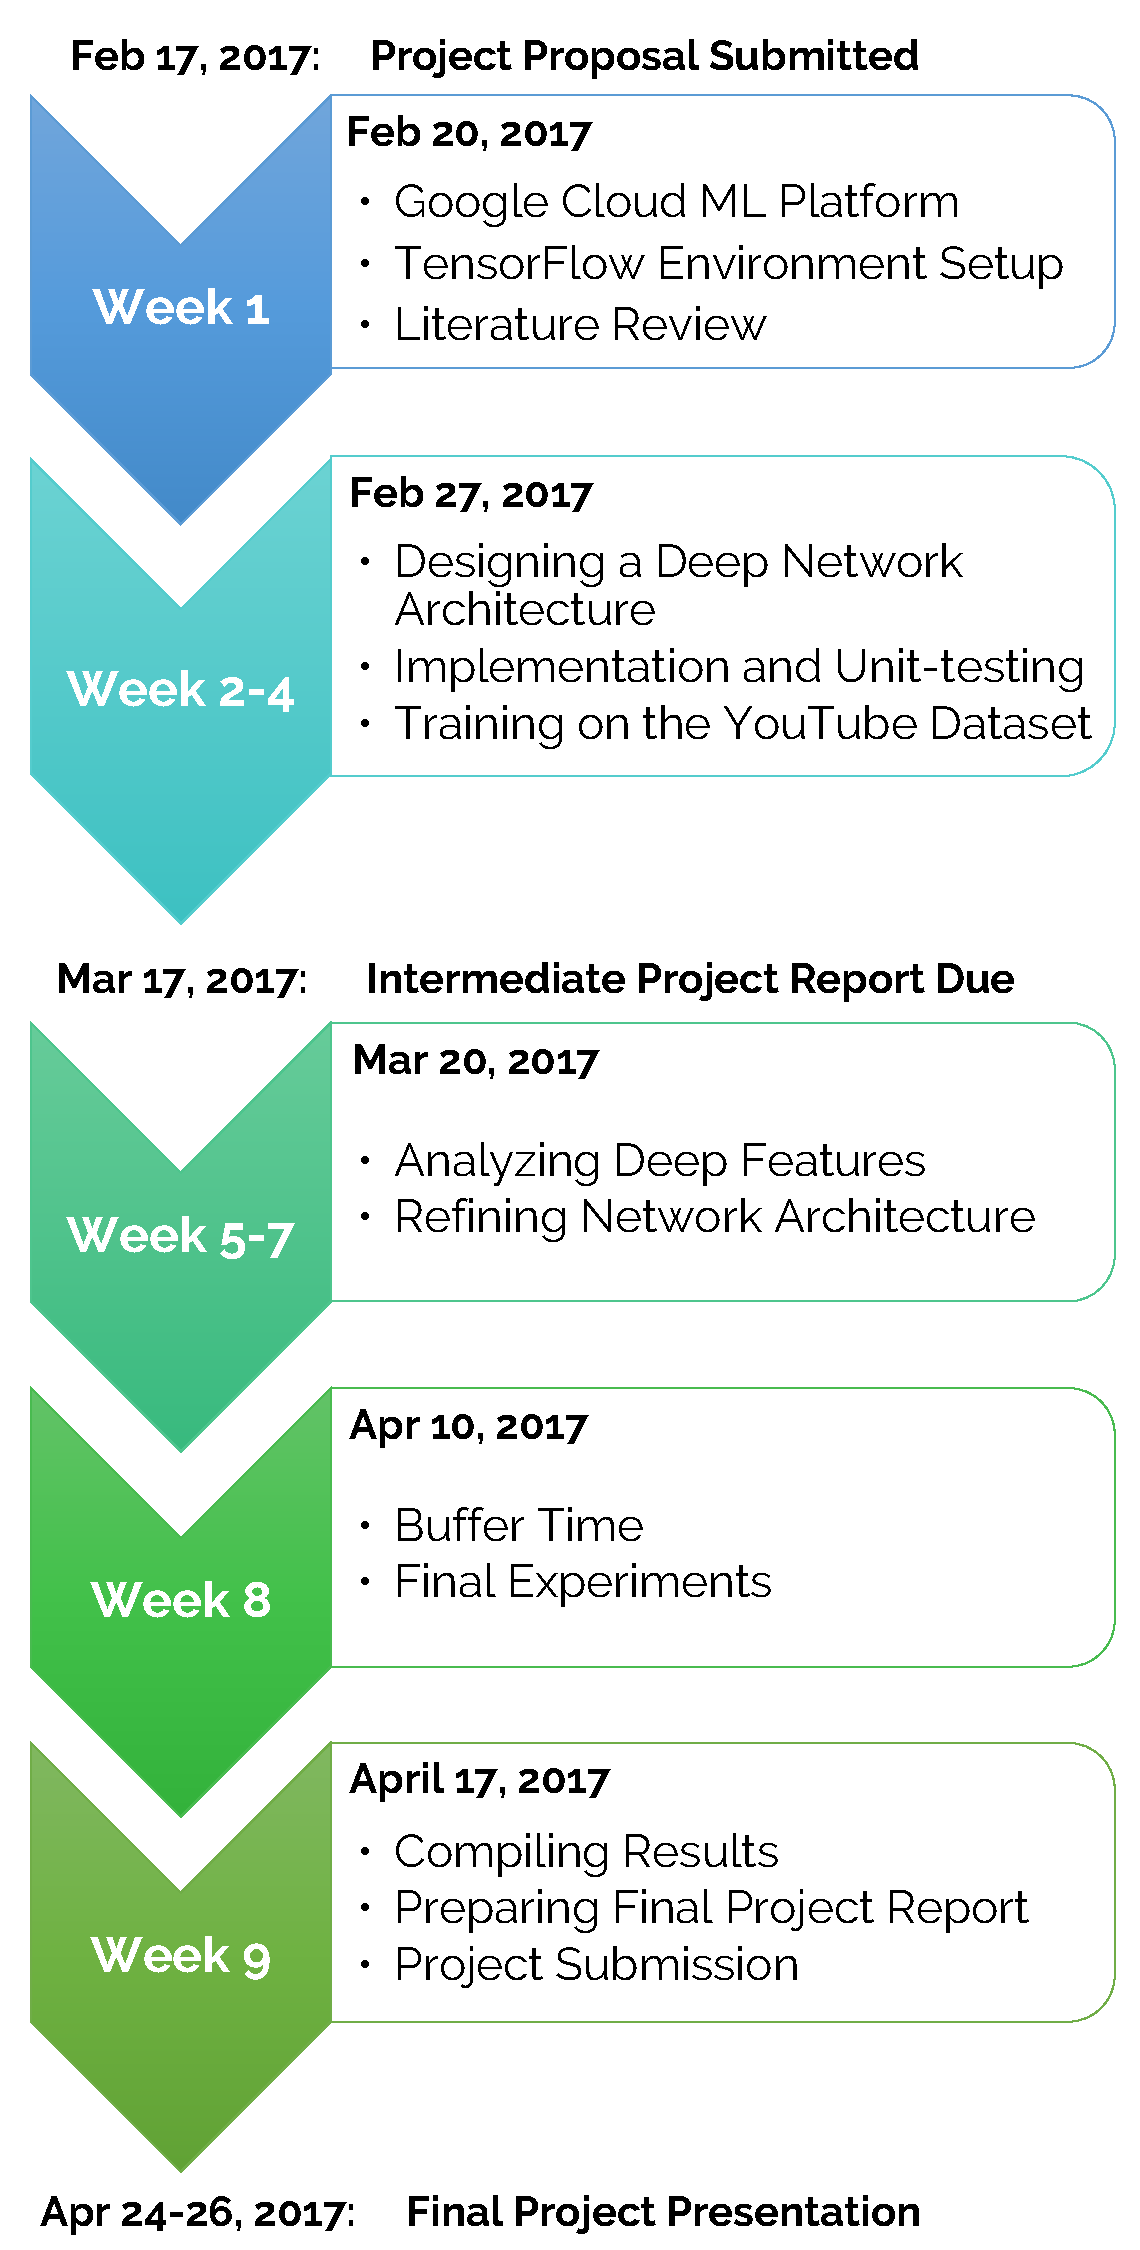
\includegraphics[width=0.87\linewidth]{timeline.pdf}
    \caption{Timeline presenting the targeted milestones in the project.}
    \label{fig:timeline}
\end{figure}

\section{Dataset}
The dataset is provided by Youtube in the Google Cloud \& Youtube-8M Video Understanding Challenge website\footnote{\url{https://research.google.com/youtube8m/download.html}}. The Youtube8m dataset contains both video level and frame level (1 sec. granularity) visual as well as audio features for 8Million videos belonging to 4000+ classes. Inception-V3 image annotation model~\cite{szegedy2016rethinking}, trained on ImageNet database~\cite{deng2009imagenet}, was used to extract the visual features from the bottleneck layer which is 2048 dimensional, and VGG based acoustic model was used to extract the audio features. In the case of frame-level features, these visual and audio representations extracted from each frame are PCAed and quantized to result in a 1024-dimensional visual feature, and 128-dimensional audio feature. For video-level features, these frame-level features have been averaged out. Fig.~\ref{fig:top20} presents the most frequent top-20 class labels in the database.

\begin{figure}[t]
    \centering
    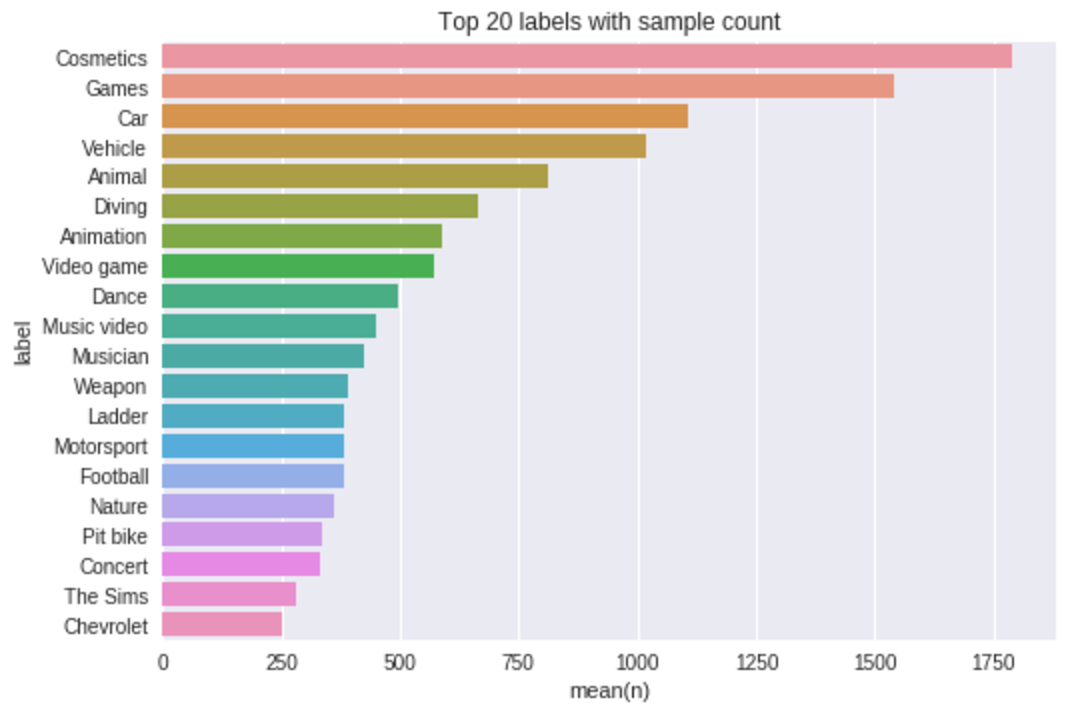
\includegraphics[width=\linewidth]{top20.png}
    \caption{Top-20 frequent class labels in Youtube-8M dataset.}
    \label{fig:top20}
\end{figure}

\section{Current Progress}
\subsection{Environment Setup}
Google provides a \$300 worth credit for competition participants to use their Google Cloud ML Platform. This platform provides an environment for accessing the large training and testing files, writing code in tensorflow, submitting training/testing jobs on their GPU resources, and downloading the predictions file for submission to the competition.

\subsection{Understanding Deep Neural Networks (CNN \& RNN)}
One of the main goals of this project is to make ourselves well-acquainted with deep neural networks, specifically Convolutional Neural Networks (CNN) and Recurrent Neural Networks (RNN). Both CNN and RNN are evolved from ordinary Neural Networks. 
\subsubsection{Convolutional Neural Networks}
CNNs are specialized neural networks for mapping 2-D and 3-D spatial information, such as in images and videos, to the desired outputs. A typical CNN architecture consists of several convolutional layers, pooling layers, fully-connected layers and typically a softmax layer at the end that is directly mapped to the output labels. Each convolutional layer maps a set of input 2-D feature maps to another set of feature maps using a shared kernel of weights (typical kernels are of sizes 3x3, 5x5, 7x7 etc.). The pooling layers remove redundancies and sub-sample the input feature maps. Thus, the convolutional layers learn low-level spatial features in images such as edges and arbitrary shapes and the fully-connected layer summarizes the low-level features into high-level shapes and objects in the input image.

\subsubsection{Recurrent Neural Networks}
Recurrent Neural Networks, on the other hand, are good for learning sequential data. As the name suggests, the output at one-time step is fed back into the network in the next time-step in a recurrent way. Thus, it tries to learn from the temporal relations in the data. As a result of the problem of vanishing gradients, a simple RNN is often unable to learn long temporal relationships in the data, concentrating on only the more recent inputs. This problem has been addressed by two prominent RNN models - the Long Short Term Memory (LSTM) and the Gated Recurrent Units (GRU). These models, in addition to the basic RNN unit, use a set of gates that control the flow of information from the current input and the previous output in the computation of the current output. They also typically use a `forget' gate to control the rate of `forgetting' past data.

\subsection{Learning Tensorflow}
TensorFlow is a python based open source library for complex numerical computations using tensors and graphs. It has been successfully applied in several deep learning applications because of the many features it offers including parallel deployment of computation to several CPUs or GPUs, data visualization toolkit etc. During the past month, we tried to learn and understand the TensorFlow library. We specifically focussed on modeling several Convolutional Neural Network architectures starting from the toy MNIST dataset to learning more diverse datasets using Inception-v3 and VGGNet architectures. We also modeled Recurrent Neural Network architectures using LSTM or GRU. In our architecture, we plan on feeding the input frame-level features from the dataset directly to a vector of RNN cells (LSTM or GRU). The last RNN cell will give the video level labels. 

\subsection{Performance Baseline}
A starter code is provided by the competition hosts to check if the environment has been setup correctly and to understand the baseline performance. With the help of the starter code, we successfully trained a LogisticModel\footnote{\url{https://github.com/google/youtube-8m/blob/master/video_level_models.py}} with L2 regularization on the video-level features (See Figs.~\ref{fig:training} and~\ref{fig:training_loss} presenting the training performance visualized using Tensorboard). A LogisticModel learns a linear projection of features to the class labels, which are then treated with a sigmoid function to result in class probabilities. We achieved an average Rank-1 accuracy of $72.4\%$ when evaluated $5000$ examples. We did not complete the full evaluation as this was only a test for correct setup. To utilize higher granularity frame level features and with the focus on to improve the performance, we are currently working on utilizing the RNN models which are known to be well-suited for sequence data such as video frames or audio signals.

\begin{figure}[t]
    \centering
    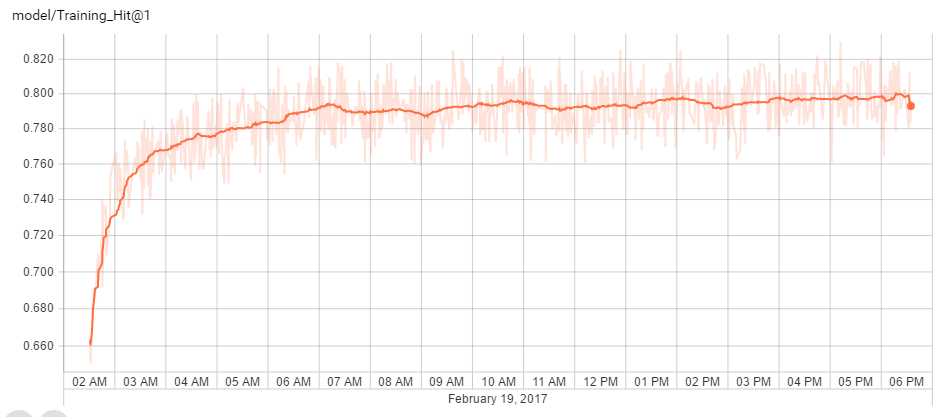
\includegraphics[width=\linewidth]{training.png}
    \caption{Tensorboard display of Rank-1 training accuracy during the training of LogisticModel.}
    \label{fig:training}
\end{figure}

\begin{figure}[t]
    \centering
    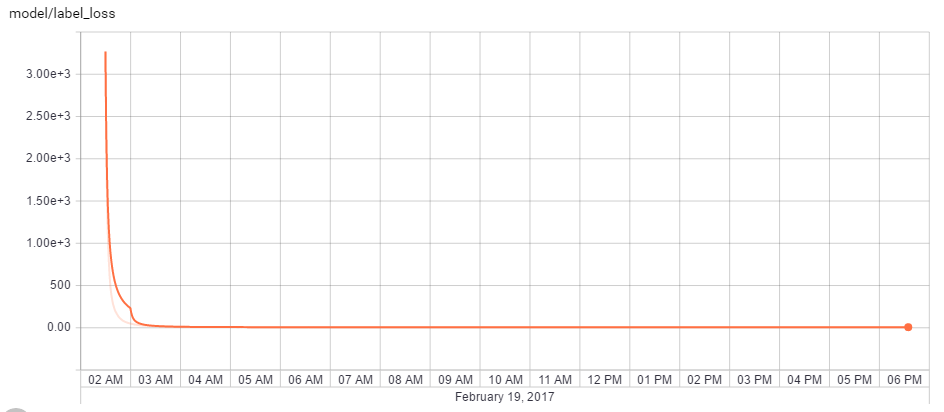
\includegraphics[width=\linewidth]{training_loss.png}
    \caption{Tensorboard display of training loss during the training of LogisticModel.}
    \label{fig:training_loss}
\end{figure}

\section{Remaining Milestones}

\subsection{Explore LSTM/GRU models}
The starter code that we tried implemented a very basic logistic model using the video-level features. We plan to implement an RNN model using both video as well as frame-level features to exploit the temporal nature of the input. Since the input dataset already consists of features trained using CNN and quantized after PCA, they represent high-level spatial information from each frame. This amounts to feeding object-level information to the RNN in order to understand the class labels associated with the videos.

\subsection{Utilizing Audio Features}
We will explore the performance of RNN models trained on the audio features independently and one concatenated with visual features, to understand the usefulness of audio features.

\subsection{Model FineTuning}
As with any machine learning model, we will fine-tune our model hyper-parameters using cross-validation with the provided validation set. These hyper parameters include the number of parallel RNN cells in the architecture, learning rate, dropout (regularization), loss function, etc. We plan to perform sufficient number of trials on the Google Cloud ML platform in order to optimize the hyper-parameters.

\subsection{Score Level Fusion}
We will explore the possibility of fusing multiple RNN models based on visual and audio features at score level to investigate if fusion can help in improving the overall performance. 


\bibliographystyle{unsrt}
\bibliography{ml_bib}  

\end{document}
